% =====================================================================
% Lösungsteil zu Kapitel 1 (Analysis) – Lösungen zu Ü 1.1 bis Ü 1.38
% Steht am Ende des Buches hinter dem Anhang.
% Alle Ergebnisse wurden mit SymPy nachgerechnet.
% =====================================================================
\Loesungskapitel{Lösungen zur Analysis}

\Uebungsabschnitt{Lokales und globales Differenzieren}

\begin{loesung}{1.1}{Änderungsrate und h-Methode}
\begin{enumerate}[label=\alph*)]
  \item \textit{Verfahren:} Die mittlere Änderungsrate ist der Differenzenquotient (Steigung der Sekante).
  \[f(1) = 1-2+3 = 2,\qquad f(4) = 16-8+3 = 11\]
  \[m_S = \dfrac{f(4)-f(1)}{4-1} = \dfrac{11-2}{3} = 3\]
  Die mittlere Änderungsrate von $f$ in $[1;4]$ beträgt $3$.
  \item \textit{Verfahren:} h-Methode, d.\,h. Grenzwert des Differenzenquotienten $f'(x_0)=\lim\limits_{h\longrightarrow 0}\dfrac{f(x_0+h)-f(x_0)}{h}$.
  \begin{align*}
    f(2+h) &= (2+h)^2-2(2+h)+3 = 4+4h+h^2-4-2h+3 = h^2+2h+3\\
    f(2) &= 3\\
    \dfrac{f(2+h)-f(2)}{h} &= \dfrac{h^2+2h}{h} = h+2 \quad (h\neq 0)\\
    f'(2) &= \lim\limits_{h\longrightarrow 0}(h+2) = 2
  \end{align*}
  \item \textit{Begründung:} Parallele Geraden haben dieselbe Steigung. Gesucht ist also $x_0$ mit $f'(x_0)=m_S=3$.\\
  Mit der Potenz-, Faktor- und Summenregel gilt $f'(x) = 2x-2$.
  \[2x_0-2 = 3 \quad\Longleftrightarrow\quad x_0 = \dfrac{5}{2}\]
  Die Stelle $x_0=\frac{5}{2}$ liegt im Intervall $[1;4]$. Die Tangente in $\left(\frac{5}{2}\big|f(\frac{5}{2})\right)$ verläuft parallel zur Sekante.
\end{enumerate}
\end{loesung}

\begin{loesung}{1.2}{Stetigkeit und Differenzierbarkeit}
\begin{enumerate}[label=\alph*)]
  \item \textit{Verfahren:} h-Methode mit links- und rechtsseitigem Grenzwert, denn der Betrag wird für $h<0$ und $h>0$ unterschiedlich aufgelöst. Es ist $f(3)=1$ und $f(3+h) = |h|+1$.
  \begin{align*}
    h<0:&\quad \dfrac{f(3+h)-f(3)}{h} = \dfrac{|h|}{h} = \dfrac{-h}{h} = -1 \;\longrightarrow\; -1\\
    h>0:&\quad \dfrac{f(3+h)-f(3)}{h} = \dfrac{|h|}{h} = \dfrac{h}{h} = 1 \;\longrightarrow\; 1
  \end{align*}
  Der linksseitige Grenzwert $-1$ und der rechtsseitige Grenzwert $1$ stimmen nicht überein. Der Grenzwert des Differenzenquotienten existiert also nicht, und $f$ ist an der Stelle $x_0=3$ \textbf{nicht differenzierbar}.\\
  \textit{Bedeutung:} $G_f$ hat im Punkt $(3|1)$ einen \glqq Knick\grqq{}. Von links kommend hat der Graph die Steigung $-1$, nach rechts die Steigung $1$. Dort lässt sich keine eindeutige Tangente anlegen.
  \item \textit{Begründung:} $f$ ist an $x_0$ stetig, wenn der Grenzwert von $f(x)$ für $x\longrightarrow x_0$ existiert und gleich $f(x_0)$ ist.\\
  Für $x\longrightarrow 3$ (von links wie von rechts) gilt $|x-3|\longrightarrow 0$, also $f(x) = |x-3|+1\longrightarrow 1 = f(3)$. Damit ist $f$ an der Stelle $3$ stetig. Der Graph lässt sich dort \glqq ohne Absetzen\grqq{} zeichnen.
  \item \textit{Stetigkeit:} Links- und rechtsseitiger Grenzwert müssen mit $g(2)$ übereinstimmen.
  \[\lim\limits_{x\longrightarrow 2^-} x^2 = 4 = g(2),\qquad \lim\limits_{x\longrightarrow 2^+}(ax+b) = 2a+b \quad\Longrightarrow\quad 2a+b = 4 \quad\text{(I)}\]
  \textit{Differenzierbarkeit:} Die Steigungen beider Teilfunktionen müssen an der Stelle $2$ übereinstimmen.
  \[(x^2)' = 2x \;\Rightarrow\; 2\cdot 2 = 4,\qquad (ax+b)' = a \quad\Longrightarrow\quad a = 4 \quad\text{(II)}\]
  (II) in (I): $8+b=4$, also $b=-4$. Für $a=4$ und $b=-4$ ist $g$ an der Stelle $2$ stetig und differenzierbar. Die Gerade $y=4x-4$ ist dann genau die Tangente an die Parabel im Punkt $(2|4)$.
\end{enumerate}
\end{loesung}

\begin{loesung}{1.3}{Lineare Transformation}
\textit{Grundlage:} Merkekasten \glqq Allgemeine Darstellung der Linearen Transformationen\grqq.
\begin{enumerate}[label=\alph*)]
  \item Ausgehend von $y=x^2$ entsteht $G_g$ durch
  \begin{enumerate}[label=\arabic*.]
    \item Verschiebung um $1$ in negative $x$-Richtung (nach links), denn $x$ wird durch $x-(-1)=x+1$ ersetzt,
    \item Streckung in Richtung der $y$-Achse mit dem Faktor $2$,
    \item Spiegelung an der $x$-Achse (Vorzeichen $-$ vor dem Faktor $2$),
    \item Verschiebung um $3$ in Richtung der $y$-Achse nach oben.
  \end{enumerate}
  Der Graph ist eine nach unten geöffnete, gestreckte Parabel mit dem Scheitel $S(-1|3)$.
  \item Spiegelung an der $y$-Achse: $x$ wird durch $-x$ ersetzt, $f(-x) = \sqrt{-x}$.\\
  Verschiebung um $2$ nach oben: $+2$ zum Funktionsterm.
  \[k(x) = \sqrt{-x}+2\]
  Der Radikand darf nicht negativ sein: $-x\geq 0 \Longleftrightarrow x\leq 0$. Also ist $\mathds{D}_k = ]-\infty;0]$.
  \item Nach dem Merkekasten entsteht der Graph von $x\mapsto h(a\cdot x)$ mit $a>0$ aus $G_h$ durch Stauchung bzw. Streckung in Richtung der $x$-Achse mit dem Faktor $\frac{1}{a}$. Aus $\frac{1}{a}=\frac{1}{2}$ folgt $a=2$.
  \[\tilde{h}(x) = \sin{(2x)}\]
  Periode: $p = \dfrac{2\pi}{2} = \pi$. Die Periode halbiert sich von $2\pi$ auf $\pi$.
\end{enumerate}
\end{loesung}

\begin{loesung}{1.4}{Newton-Verfahren}
\begin{enumerate}[label=\alph*)]
  \item \textit{Existenz:} $f$ ist als ganzrationale Funktion stetig. Es gilt
  \[f(0) = -1 < 0 \qquad\text{und}\qquad f(1) = 1+1-1 = 1 > 0.\]
  Weil $f$ stetig ist und das Vorzeichen zwischen $0$ und $1$ wechselt, muss $G_f$ die $x$-Achse in $]0;1[$ schneiden.\\
  \textit{Eindeutigkeit:} $f'(x) = 3x^2+1 > 0$ für alle $x\in\mathds{R}$. Nach dem Satz \glqq Bedingung für die Monotonie\grqq{} ist $f$ in ganz $\mathds{R}$ streng monoton wachsend und kann deshalb höchstens eine Nullstelle haben.\\
  Zusammen: $f$ hat genau eine Nullstelle, und diese liegt in $[0;1]$.
  \item \textit{Verfahren:} Newton-Iteration $x_{n+1} = x_n - \dfrac{f(x_n)}{f'(x_n)}$ mit $f'(x)=3x^2+1$.
  \begin{align*}
    x_1 &= 1 - \dfrac{f(1)}{f'(1)} = 1-\dfrac{1}{4} = 0{,}75 = 0{,}7500\\
    x_2 &= 0{,}75 - \dfrac{f(0{,}75)}{f'(0{,}75)} = 0{,}75 - \dfrac{0{,}171875}{2{,}6875} = \dfrac{59}{86} \approx 0{,}6860
  \end{align*}
  (Zum Vergleich: Die Nullstelle ist $x_N\approx 0{,}6823$.)
  \item $g'(x) = 3x^2-3$, also $g'(1) = 0$. Die Tangente an $G_g$ im Startpunkt $(1|-2)$ verläuft waagrecht und schneidet die $x$-Achse nicht. Im Newton-Verfahren müsste man durch $g'(1)=0$ teilen. Der Wert $x_1$ ist also nicht definiert und das Verfahren bricht ab.
\end{enumerate}
\end{loesung}

\Uebungsabschnitt{Kurvendiskussion}

\begin{loesung}{1.5}{Tangente und Normale}
Ableitung (Potenz-, Faktor- und Summenregel): $f'(x) = 3x^2-6x$.
\begin{enumerate}[label=\alph*)]
  \item $f(1) = 1-3+4 = 2$, also $P(1|2)$. Steigung: $f'(1) = 3-6 = -3$.\\
  \textit{Verfahren:} Tangentengleichung $y = f'(x_0)\cdot(x-x_0)+f(x_0)$.
  \[t:\ y = -3\cdot(x-1)+2 = -3x+5\]
  \item \textit{Definition der Normalen:} $m_{\text{Normale}} = -\dfrac{1}{m_{\text{Tangente}}} = -\dfrac{1}{-3} = \dfrac{1}{3}$.
  \[n:\ y = \dfrac{1}{3}(x-1)+2 = \dfrac{1}{3}x+\dfrac{5}{3}\]
  \item Parallele Geraden haben gleiche Steigung. Gesucht sind die Stellen mit $f'(x)=9$.
  \begin{align*}
    3x^2-6x &= 9 \quad\Big|\,:3\\
    x^2-2x-3 &= 0\\
    (x-3)(x+1) &= 0 \quad\Longrightarrow\quad x_1 = -1,\ x_2 = 3
  \end{align*}
  $f(-1) = -1-3+4 = 0$ und $f(3) = 27-27+4 = 4$. Die gesuchten Punkte sind $(-1|0)$ und $(3|4)$.
\end{enumerate}
\end{loesung}

\begin{loesung}{1.6}{Monotonie, Extrema und Krümmung}
\begin{enumerate}[label=\alph*)]
  \item Ausklammern und binomische Formel:
  \[f(x) = x\cdot(x^2-6x+9) = x\cdot(x-3)^2\]
  Nach dem Satz vom Nullprodukt sind die Nullstellen $x_1=0$ (einfach, $G_f$ schneidet die $x$-Achse) und $x_2=3$ (doppelt, $G_f$ berührt die $x$-Achse).
  \item $f'(x) = 3x^2-12x+9 = 3\cdot(x^2-4x+3) = 3\cdot(x-1)(x-3)$, Nullstellen von $f'$: $1$ und $3$.
  \begin{center}\begin{tabular}{||c|c|c|c|c|c||}
    \hline
    $x$ & $x<1$ & $x=1$ & $1<x<3$ & $x=3$ & $x>3$\\
    \hline\hline
    $3\cdot(x-1)$ & $-$ & $0$ & $+$ & $+$ & $+$\\
    \hline
    $(x-3)$ & $-$ & $-$ & $-$ & $0$ & $+$\\
    \hline
    $f'(x)$ & $+$ & $0$ & $-$ & $0$ & $+$\\
    \hline
    $G_f$ & smw & HoP & smf & TiP & smw\\
    \hline
  \end{tabular}\end{center}
  Nach dem Satz \glqq Bedingung für die Monotonie\grqq{} ist $G_f$ in $]-\infty;1]$ und in $[3;\infty[$ streng monoton wachsend, in $[1;3]$ streng monoton fallend. Vorzeichenwechsel von $f'$ von $+$ nach $-$ bei $x=1$ ergibt einen Hochpunkt, von $-$ nach $+$ bei $x=3$ einen Tiefpunkt.
  \[f(1) = 1-6+9 = 4 \;\Longrightarrow\; HoP(1|4),\qquad f(3) = 0 \;\Longrightarrow\; TiP(3|0)\]
  \item $f''(x) = 6x-12 = 6\cdot(x-2)$. Nach dem Kriterium der Krümmung gilt:
  \begin{itemize}
    \item $x<2$: $f''(x)<0$, $G_f$ ist rechtsgekrümmt.
    \item $x>2$: $f''(x)>0$, $G_f$ ist linksgekrümmt.
  \end{itemize}
  Bei $x=2$ wechselt $f''$ das Vorzeichen, dort liegt ein Wendepunkt. Mit $f(2) = 8-24+18 = 2$ folgt $WP(2|2)$.
  \item $f'(2) = 12-24+9 = -3$. Tangentengleichung:
  \[w:\ y = -3\cdot(x-2)+2 = -3x+8\]
  \item Zusätzliche Werte für die Skizze: $f(-0{,}5) = -6{,}125$ und $f(4{,}5) = 10{,}125$.
  \begin{center}
  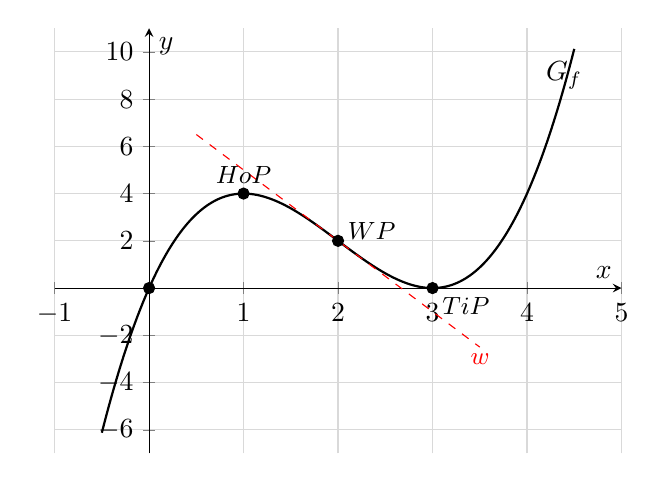
\begin{tikzpicture}
  \begin{axis}[ticklabel style={fill=none}, every tick label/.append style={fill=none},
      axis lines=middle, xmin=-1, xmax=5, ymin=-7, ymax=11,
      x=1.2cm, y=0.3cm, xtick={-1,0,...,5}, ytick={-6,-4,...,10},
      xlabel=$x$, ylabel=$y$, grid=major, grid style={gray!30}]
    \addplot[thick, samples=200, domain=-0.5:4.5]{x^3-6*x^2+9*x};
    \addplot[dashed, red, domain=0.5:3.5]{-3*x+8};
    \addplot[only marks, mark=*] coordinates {(1,4) (3,0) (2,2) (0,0)};
    \node[above] at (axis cs:1,4) {\small $HoP$};
    \node[below right] at (axis cs:3,0) {\small $TiP$};
    \node[right] at (axis cs:2,2.4) {\small $WP$};
    \node[right] at (axis cs:4.1,9) {$G_f$};
    \node[red, right] at (axis cs:3.3,-3) {\small $w$};
  \end{axis}
  \end{tikzpicture}
  \end{center}
\end{enumerate}
\end{loesung}

\begin{loesung}{1.7}{Ausführliche Kurvendiskussion}
\textit{Vorgehen:} Schritte der ausführlichen Kurvendiskussion (Merkekasten).
\begin{enumerate}[label=\alph*)]
  \item $f$ ist ganzrational, also ist $\mathds{D}_{\text{max}} = \mathds{R}$.\\
  \textit{Symmetrie:} $f(-x) = \frac{1}{4}x^4+x^3$. Das ist weder $f(x)$ noch $-f(x)$, weil der Term gerade ($x^4$) und ungerade ($x^3$) Exponenten enthält. Zum Beispiel ist $f(1)=-\frac{3}{4}$, aber $f(-1)=\frac{5}{4}$. $G_f$ ist weder achsensymmetrisch zur $y$-Achse noch punktsymmetrisch zum Ursprung.
  \item \textit{Randverhalten:} Für $|x|\longrightarrow\infty$ bestimmt der Summand mit dem höchsten Exponenten, $\frac{1}{4}x^4$, das Verhalten:
  \[\lim\limits_{x\longrightarrow -\infty} f(x) = +\infty,\qquad \lim\limits_{x\longrightarrow +\infty} f(x) = +\infty\]
  \textit{Achsenpunkte:} $f(0) = 0$, also $S_y(0|0)$. Nullstellen:
  \[\dfrac{1}{4}x^4-x^3 = \dfrac{1}{4}x^3\cdot(x-4) = 0 \quad\Longrightarrow\quad x_1 = 0 \text{ (dreifach)},\ x_2 = 4\]
  Gemeinsame Punkte mit den Achsen: $O(0|0)$ und $N(4|0)$.
  \item $f'(x) = x^3-3x^2 = x^2\cdot(x-3)$. Notwendige Bedingung $f'(x)=0$: $x=0$ (doppelt) oder $x=3$.\\
  Weil $x^2\geq 0$ ist, hat $f'(x)$ für $x\neq 0$ dasselbe Vorzeichen wie $(x-3)$:
  \begin{center}\begin{tabular}{||c|c|c|c|c|c||}
    \hline
    $x$ & $x<0$ & $x=0$ & $0<x<3$ & $x=3$ & $x>3$\\
    \hline\hline
    $f'(x)$ & $-$ & $0$ & $-$ & $0$ & $+$\\
    \hline
    $G_f$ & smf & Terrassenpunkt & smf & TiP & smw\\
    \hline
  \end{tabular}\end{center}
  \begin{itemize}
    \item $x=0$: $f'(0)=0$, aber kein Vorzeichenwechsel von $f'$ (doppelte Nullstelle). Nach dem Kriterium für einen Terrassenpunkt liegt im Ursprung $O(0|0)$ ein \textbf{Terrassenpunkt}.
    \item $x=3$: Vorzeichenwechsel von $-$ nach $+$, also Tiefpunkt. $f(3) = \frac{81}{4}-27 = -\frac{27}{4}$, also $TiP\left(3\big|-\frac{27}{4}\right)$.
  \end{itemize}
  \item $f''(x) = 3x^2-6x = 3x\cdot(x-2)$, Nullstellen $x=0$ und $x=2$. Beide sind einfach, $f''$ wechselt dort also das Vorzeichen ($f''>0$ für $x<0$, $f''<0$ für $0<x<2$, $f''>0$ für $x>2$).\\
  Damit gibt es zwei Wendepunkte: $W_1(0|0)$, der zugleich der Terrassenpunkt ist, und $W_2(2|-4)$ wegen $f(2) = 4-8 = -4$.
  \item $f$ ist stetig, besitzt nur den einen Tiefpunkt und strebt an beiden Rändern gegen $+\infty$. Der Tiefpunkt ist daher der absolut tiefste Punkt, und alle Werte ab $-\frac{27}{4}$ werden angenommen:
  \[W_f = \left[-\dfrac{27}{4};\infty\right[\]
  \begin{center}
  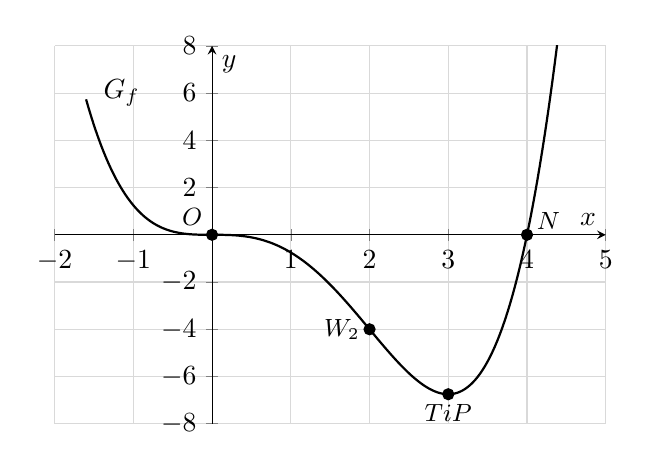
\begin{tikzpicture}
  \begin{axis}[ticklabel style={fill=none}, every tick label/.append style={fill=none},
      axis lines=middle, xmin=-2, xmax=5, ymin=-8, ymax=8,
      x=1cm, y=0.3cm, xtick={-2,-1,...,5}, ytick={-8,-6,...,8},
      xlabel=$x$, ylabel=$y$, grid=major, grid style={gray!30}]
    \addplot[thick, samples=200, domain=-1.6:4.7]{0.25*x^4-x^3};
    \addplot[only marks, mark=*] coordinates {(0,0) (3,-6.75) (2,-4) (4,0)};
    \node[above left] at (axis cs:0,0) {\small $O$};
    \node[below] at (axis cs:3,-6.75) {\small $TiP$};
    \node[left] at (axis cs:2,-4) {\small $W_2$};
    \node[right] at (axis cs:4,0.6) {\small $N$};
    \node[right] at (axis cs:-1.5,6) {$G_f$};
  \end{axis}
  \end{tikzpicture}
  \end{center}
\end{enumerate}
\end{loesung}

\begin{loesung}{1.8}{Graph der Ableitungsfunktion}
\textit{Grundidee:} Das Vorzeichen von $f'$ (Lage von $G_{f'}$ oberhalb oder unterhalb der $x$-Achse) gibt die Monotonie von $f$ an. Die Steigung von $G_{f'}$ (also $f''$) gibt die Krümmung von $G_f$ an.
\begin{enumerate}[label=\alph*)]
  \item $f'$ hat die Nullstellen $-1$ und $3$, und an beiden wechselt das Vorzeichen:
  \begin{itemize}
    \item $x=-1$: $G_{f'}$ verläuft links von $-1$ oberhalb, rechts davon unterhalb der $x$-Achse. VZW von $+$ nach $-$, also hat $f$ bei $x=-1$ ein \textbf{Maximum} (Hochpunkt).
    \item $x=3$: VZW von $-$ nach $+$, also hat $f$ bei $x=3$ ein \textbf{Minimum} (Tiefpunkt).
  \end{itemize}
  \item Eine Wendestelle von $f$ ist eine Extremstelle von $f'$. Die Parabel $G_{f'}$ hat ihren Scheitel (Tiefpunkt) wegen der Symmetrie in der Mitte zwischen den Nullstellen, also bei $x=\frac{-1+3}{2}=1$. Links davon fällt $G_{f'}$ ($f''<0$, $G_f$ rechtsgekrümmt), rechts davon steigt $G_{f'}$ ($f''>0$, $G_f$ linksgekrümmt). Die Wendestelle von $f$ ist $x=1$.
  \item Im Intervall $]-1;3[$ verläuft $G_{f'}$ unterhalb der $x$-Achse, d.\,h. $f'(x)<0$. Nach dem Satz \glqq Bedingung für die Monotonie\grqq{} ist $f$ in $[-1;3]$ streng monoton fallend. Wegen $0<3$ folgt $f(3)<f(0)$. Die Aussage ist \textbf{wahr}.
  \item Die Skizze muss enthalten: Hochpunkt bei $x=-1$, Wendepunkt bei $x=1$, Tiefpunkt bei $x=3$, Verlauf durch den Ursprung. Die Steigung im Ursprung ist $f'(0)=-1{,}5$, die Steigung im Wendepunkt $f'(1)=-2$. Für die eingezeichnete Kurve wurde der Term $f(x) = \frac{1}{6}x^3-\frac{1}{2}x^2-\frac{3}{2}x$ verwendet. Er erfüllt $f'(x)=0{,}5(x+1)(x-3)$ und $f(0)=0$. Damit liegen die besonderen Punkte bei $HoP\left(-1\big|\frac{5}{6}\right)$, $WP\left(1\big|-\frac{11}{6}\right)$ und $TiP\left(3\big|-\frac{9}{2}\right)$.
  \begin{center}
  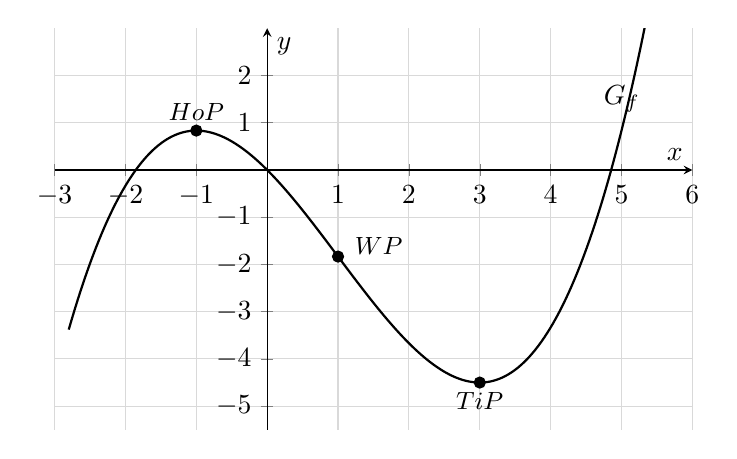
\begin{tikzpicture}
  \begin{axis}[ticklabel style={fill=none}, every tick label/.append style={fill=none},
      axis lines=middle, xmin=-3, xmax=6, ymin=-5.5, ymax=3,
      x=0.9cm, y=0.6cm, xtick={-3,-2,...,6}, ytick={-5,-4,...,2},
      xlabel=$x$, ylabel=$y$, grid=major, grid style={gray!30}]
    \addplot[thick, samples=200, domain=-2.8:5.6]{x^3/6-x^2/2-1.5*x};
    \addplot[only marks, mark=*] coordinates {(-1,0.8333) (1,-1.8333) (3,-4.5)};
    \node[above] at (axis cs:-1,0.83) {\small $HoP$};
    \node[right] at (axis cs:1.1,-1.6) {\small $WP$};
    \node[below] at (axis cs:3,-4.5) {\small $TiP$};
    \node[left] at (axis cs:5.4,1.5) {$G_f$};
  \end{axis}
  \end{tikzpicture}
  \end{center}
\end{enumerate}
\end{loesung}

\Uebungsabschnitt{Stammfunktion}

\begin{loesung}{1.9}{Stammfunktionen ganzrationaler Funktionen}
\textit{Grundlage:} Satz \glqq Stammfunktion der Potenzfunktion\grqq{}, $x^n \mapsto \frac{1}{n+1}x^{n+1}$, sowie die Faktor- und Summenregel für Stammfunktionen.
\begin{enumerate}[label=\alph*)]
  \item \[F(x) = x^3-2x^2+x,\qquad G(x) = \dfrac{1}{12}x^6-\dfrac{1}{2}x^2,\qquad H(x) = \dfrac{a^2}{4}x^4+2a\cdot x\]
  Bei $h$ ist $a$ ein konstanter Parameter. $a^2$ wird wie ein Faktor behandelt, $2a$ wie eine Konstante (Stammfunktion $2a\cdot x$).\\
  \textit{Probe:} $F'(x) = 3x^2-4x+1 = f(x)$, analog für $G$ und $H$.
  \item Alle Stammfunktionen von $f$ haben die Form $F(x) = 2x^3-2x+c$ mit $c\in\mathds{R}$. Die Bedingung, dass der Graph durch $P(1|3)$ verläuft, ergibt:
  \[F(1) = 2-2+c = 3 \quad\Longrightarrow\quad c = 3,\qquad F(x) = 2x^3-2x+3\]
  \item Nach der Summenregel und weil die Ableitung einer Konstanten null ist, gilt
  \[G'(x) = F'(x)+0 = f(x).\]
  Also ist $G$ ebenfalls eine Stammfunktion von $f$. Der Graph von $G$ entsteht aus dem Graphen von $F$ durch Verschiebung um $c$ in Richtung der $y$-Achse. An jeder Stelle $x$ haben beide Graphen dieselbe Steigung, sie verlaufen also \glqq parallel\grqq{} in $y$-Richtung.
\end{enumerate}
\end{loesung}

\Uebungsabschnitt{Funktionenscharen}

\begin{loesung}{1.10}{Funktionenschar und Ortskurve}
Ableitungen: $f_k'(x) = 3x^2-k$, $f_k''(x) = 6x$, $f_k'''(x) = 6$.
\begin{enumerate}[label=\alph*)]
  \item $f_k(x) = x\cdot(x^2-k) = 0 \Longleftrightarrow x=0$ oder $x^2=k$ (Satz vom Nullprodukt).
  \begin{itemize}
    \item $k>0$: $x^2=k$ hat die Lösungen $\pm\sqrt{k}$. Es gibt \textbf{drei} Nullstellen: $-\sqrt{k}$, $0$ und $\sqrt{k}$.
    \item $k=0$: $f_0(x) = x^3$ hat nur die (dreifache) Nullstelle $0$, also \textbf{eine} Nullstelle.
    \item $k<0$: $x^2=k$ hat keine Lösung, also \textbf{eine} Nullstelle ($x=0$).
  \end{itemize}
  \item $f_k''(0) = 0$ und $f_k'''(0) = 6\neq 0$ (gleichwertig: $f_k''(x)=6x$ wechselt bei $0$ das Vorzeichen). Wegen $f_k(0)=0$ ist der Ursprung für jedes $k$ Wendepunkt. Steigung der Wendetangente: $m = f_k'(0) = -k$.
  \item $f_k'(x) = 0 \Longleftrightarrow x^2 = \dfrac{k}{3} \Longleftrightarrow x = \pm\sqrt{\dfrac{k}{3}}$ (für $k>0$ reell).
  \begin{itemize}
    \item $f_k''\left(-\sqrt{\frac{k}{3}}\right) = -6\sqrt{\frac{k}{3}} < 0$, also Hochpunkt bei $x_H = -\sqrt{\frac{k}{3}}$.
    \item $f_k''\left(\sqrt{\frac{k}{3}}\right) = 6\sqrt{\frac{k}{3}} > 0$, also Tiefpunkt bei $x_T = \sqrt{\frac{k}{3}}$.
  \end{itemize}
  \item \textit{Verfahren:} Merkekasten \glqq Bestimmung der Ortskurve besonderer Punkte\grqq{}, d.\,h. $x$-Koordinate nach $k$ auflösen und in die $y$-Koordinate einsetzen.\\
  Für den Hochpunkt gilt $x = -\sqrt{\frac{k}{3}}$ mit $x<0$. Quadrieren liefert $x^2 = \frac{k}{3}$, also $k = 3x^2$. Einsetzen in $y = f_k(x)$:
  \[y = x^3 - 3x^2\cdot x = -2x^3\]
  Ortskurve der Hochpunkte: $y = -2x^3$ mit $x<0$ (wegen $k>0$).
\end{enumerate}
\end{loesung}

\Uebungsabschnitt{Untersuchung von speziellen Funktionen}

\begin{loesung}{1.11}{Gebrochen-rationale Funktion}
\begin{enumerate}[label=\alph*)]
  \item Der Nenner wird null für $x=2$, also ist $\mathds{D}_{\text{max}} = \mathds{R}\setminus\{2\}$.\\
  Nullstellen: Zähler gleich null und Nenner ungleich null.
  \[x^2-4x+3 = (x-1)(x-3) = 0 \quad\Longrightarrow\quad x_1 = 1,\ x_2 = 3\]
  Beide liegen in $\mathds{D}_f$. Die Nullstellen sind $1$ und $3$.
  \item Rechte Seite auf den Hauptnenner bringen:
  \[x-2-\dfrac{1}{x-2} = \dfrac{(x-2)^2-1}{x-2} = \dfrac{x^2-4x+4-1}{x-2} = \dfrac{x^2-4x+3}{x-2} = f(x)\]
  \item \textit{Definitionslücke:} Der Zähler hat bei $x=2$ den Wert $4-8+3=-1\neq 0$, also liegt ein Pol vor. Mit der Darstellung aus b):
  \[x\longrightarrow 2^-:\ x-2\longrightarrow 0^-,\ -\dfrac{1}{x-2}\longrightarrow +\infty \;\Rightarrow\; f(x)\longrightarrow+\infty\]
  \[x\longrightarrow 2^+:\ x-2\longrightarrow 0^+,\ -\dfrac{1}{x-2}\longrightarrow -\infty \;\Rightarrow\; f(x)\longrightarrow-\infty\]
  Es liegt ein Pol mit Vorzeichenwechsel vor, und $x=2$ ist senkrechte Asymptote.\\
  \textit{Verhalten für $x\longrightarrow\pm\infty$:} $\dfrac{1}{x-2}\longrightarrow 0$, also
  \[\lim\limits_{x\longrightarrow\pm\infty}\big(f(x)-(x-2)\big) = \lim\limits_{x\longrightarrow\pm\infty}\left(-\dfrac{1}{x-2}\right) = 0.\]
  Nach dem Merkekasten \glqq Schräge Asymptoten\grqq{} ist $y=x-2$ schräge Asymptote, und es gilt $f(x)\longrightarrow\pm\infty$ für $x\longrightarrow\pm\infty$.\\
  Asymptoten: $x=2$ und $y=x-2$.
  \item Mit der Darstellung aus b) und $\left(-(x-2)^{-1}\right)' = (x-2)^{-2}$ (Kettenregel bzw. Potenzregel):
  \[f'(x) = 1+\dfrac{1}{(x-2)^2}\]
  Für alle $x\in\mathds{D}_f$ ist $(x-2)^2>0$, also $f'(x)>1>0$. Nach dem Satz \glqq Bedingung für die Monotonie\grqq{} ist $G_f$ in $]-\infty;2[$ und in $]2;\infty[$ jeweils streng monoton wachsend. (Auf ganz $\mathds{D}_f$ gilt das nicht, z.\,B. ist $f(1{,}9)=9{,}9 > f(2{,}1)=-9{,}9$.)
  \item $f''(x) = -\dfrac{2}{(x-2)^3}$.
  \begin{itemize}
    \item $x<2$: $(x-2)^3<0$, also $f''(x)>0$, linksgekrümmt.
    \item $x>2$: $(x-2)^3>0$, also $f''(x)<0$, rechtsgekrümmt.
  \end{itemize}
  Das Krümmungsverhalten wechselt zwar an der Stelle $2$. Ein Wendepunkt ist aber ein Punkt des Graphen, und wegen $2\notin\mathds{D}_f$ gibt es dort keinen Punkt von $G_f$. Außerdem ist $f''(x)\neq 0$ für alle $x\in\mathds{D}_f$. Also hat $G_f$ keinen Wendepunkt.
  \item Skizze mit den Nullstellen aus a) und den Asymptoten aus c):
  \begin{center}
  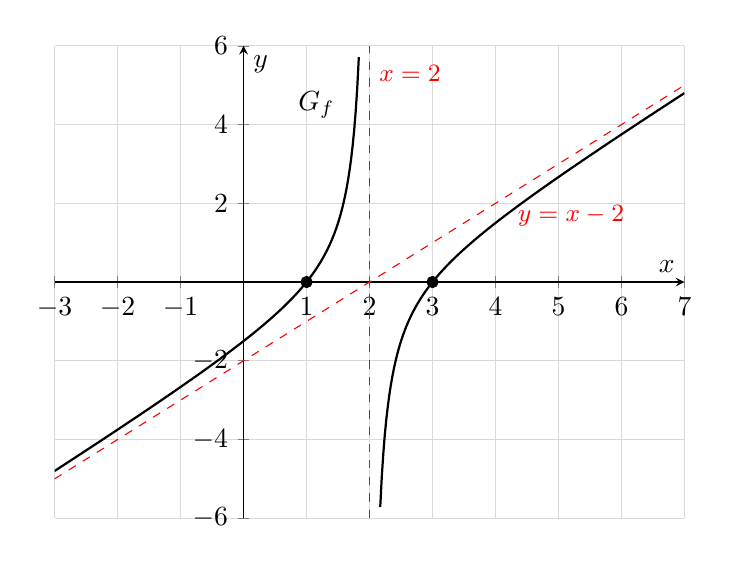
\begin{tikzpicture}
  \begin{axis}[ticklabel style={fill=none}, every tick label/.append style={fill=none},
      axis lines=middle, xmin=-3, xmax=7, ymin=-6, ymax=6,
      x=0.8cm, y=0.5cm, xtick={-3,-2,...,7}, ytick={-6,-4,...,6},
      xlabel=$x$, ylabel=$y$, grid=major, grid style={gray!30}, restrict y to domain=-7:7]
    \addplot[thick, samples=200, domain=-3:1.83]{x-2-1/(x-2)};
    \addplot[thick, samples=200, domain=2.17:7]{x-2-1/(x-2)};
    \addplot[dashed, red, domain=-3:7]{x-2};
    \draw[dashed, red] (axis cs:2,-6) -- (axis cs:2,6);
    \addplot[only marks, mark=*] coordinates {(1,0) (3,0)};
    \node[red, below right] at (axis cs:4.2,2.2) {\small $y=x-2$};
    \node[red, right] at (axis cs:2,5.3) {\small $x=2$};
    \node[left] at (axis cs:1.6,4.5) {$G_f$};
  \end{axis}
  \end{tikzpicture}
  \end{center}
\end{enumerate}
\end{loesung}

\begin{loesung}{1.12}{Definitionslücken}
\begin{enumerate}[label=\alph*)]
  \item Nenner: $x^2+x = x\cdot(x+1) = 0$ für $x=0$ und $x=-1$. Das sind die Definitionslücken, $\mathds{D}_g = \mathds{R}\setminus\{-1;0\}$.\\
  Zähler faktorisieren (3.~binomische Formel) und kürzen (für $x\neq -1$):
  \[g(x) = \dfrac{(x-1)(x+1)}{x\cdot(x+1)} = \dfrac{x-1}{x}\]
  \begin{itemize}
    \item $x=-1$: Der Faktor $(x+1)$ lässt sich kürzen. Die Definitionslücke ist \textbf{hebbar}, denn $\lim\limits_{x\longrightarrow -1} g(x) = \dfrac{-2}{-1} = 2$. Der Graph hat dort ein \glqq Loch\grqq{} im Punkt $(-1|2)$.
    \item $x=0$: Der gekürzte Zähler ist $0-1=-1\neq 0$, also liegt ein \textbf{Pol} vor.
    \[x\longrightarrow 0^-:\ \dfrac{x-1}{x}\longrightarrow\dfrac{-1}{0^-} = +\infty,\qquad x\longrightarrow 0^+:\ \dfrac{x-1}{x}\longrightarrow\dfrac{-1}{0^+} = -\infty\]
    Es ist ein Pol \textbf{mit} Vorzeichenwechsel, und $x=0$ ist senkrechte Asymptote.
  \end{itemize}
  \item Zählergrad gleich Nennergrad ($2$). Für $x\longrightarrow\pm\infty$ strebt $g(x)$ gegen den Quotienten der Koeffizienten der höchsten Potenzen, $\frac{1}{1}=1$. Mit der Summenform sieht man das direkt: $g(x) = 1-\dfrac{1}{x}\longrightarrow 1$.\\
  Die waagrechte Asymptote ist $y=1$.
\end{enumerate}
\end{loesung}

\begin{loesung}{1.13}{Umkehrfunktion und Wurzelfunktionen}
\begin{enumerate}[label=\alph*)]
  \item \textit{Umkehrbarkeit:} $f'(x) = 2(x-1) > 0$ für $x>1$. $f$ ist also in $\mathds{D}_f = [1;\infty[$ streng monoton wachsend und nach dem Kriterium für die Umkehrbarkeit umkehrbar. Anschaulich ist $G_f$ der rechte Ast einer Parabel mit Scheitel $(1|2)$. Wertemenge: $W_f = [2;\infty[$.\\
  \textit{Term der Umkehrfunktion:} Nach $x$ auflösen, danach $x$ und $y$ vertauschen.
  \begin{align*}
    y &= (x-1)^2+2 \quad\big|\,-2\\
    y-2 &= (x-1)^2 \quad\big|\,\sqrt{\phantom{x}}\ \text{(positive Wurzel, da $x-1\geq 0$)}\\
    x &= 1+\sqrt{y-2}
  \end{align*}
  \[f^{-1}(x) = 1+\sqrt{x-2},\qquad \mathds{D}_{f^{-1}} = W_f = [2;\infty[,\qquad W_{f^{-1}} = \mathds{D}_f = [1;\infty[\]
  \item Aus $y=\sqrt{9-(x-2)^2}$ folgt $y\geq 0$ und durch Quadrieren $(x-2)^2+y^2 = 9 = 3^2$. Das ist die Gleichung eines Kreises mit Mittelpunkt $M(2|0)$ und Radius $r=3$ (Merkekasten \glqq Halbkreise mit beliebigem Mittelpunkt\grqq). Wegen $y\geq 0$ ist $G_g$ der obere Halbkreis.\\
  Definitionsbereich: $9-(x-2)^2\geq 0 \Longleftrightarrow |x-2|\leq 3 \Longleftrightarrow -1\leq x\leq 5$, also $\mathds{D}_{\text{max}} = [-1;5]$.
  \item $h(2) = \sqrt{9} = 3$, also $Q(2|3)$.\\
  Kettenregel (äußere Funktion Wurzel, innere Funktion $4x+1$):
  \[h'(x) = \dfrac{1}{2\sqrt{4x+1}}\cdot 4 = \dfrac{2}{\sqrt{4x+1}},\qquad h'(2) = \dfrac{2}{3}\]
  \[t:\ y = \dfrac{2}{3}(x-2)+3 = \dfrac{2}{3}x+\dfrac{5}{3}\]
\end{enumerate}
\end{loesung}

\begin{loesung}{1.14}{Trigonometrische Funktion}
\begin{enumerate}[label=\alph*)]
  \item Vergleich mit $a\cdot\cos{(b\cdot x)}+d$: $a=2$, $b=2$, $d=1$.
  \begin{itemize}
    \item Amplitude: $|a| = 2$
    \item Periode: $p = \dfrac{2\pi}{b} = \pi$
    \item Wertemenge: Aus $-1\leq\cos{(2x)}\leq 1$ folgt $-2+1\leq f(x)\leq 2+1$. Weil $\mathds{D}_f=[0;\pi]$ genau eine Periode umfasst, werden alle diese Werte angenommen: $W_f = [-1;3]$.
  \end{itemize}
  \item \[2\cos{(2x)}+1 = 0 \quad\Longleftrightarrow\quad \cos{(2x)} = -\dfrac{1}{2}\]
  Mit $z=2x$ und $z\in[0;2\pi]$ (da $x\in[0;\pi]$) liefern die Eigenschaften der Kosinuskurve $z = \frac{2\pi}{3}$ oder $z = \frac{4\pi}{3}$. Die Nullstellen sind $x_1 = \dfrac{\pi}{3}$ und $x_2 = \dfrac{2\pi}{3}$.
  \item Kettenregel: $f'(x) = 2\cdot(-\sin{(2x)})\cdot 2 = -4\sin{(2x)}$.\\
  $f'(x) = 0 \Longleftrightarrow \sin{(2x)}=0$, mit $2x\in[0;2\pi]$ also $2x\in\{0;\pi;2\pi\}$ bzw. $x\in\{0;\frac{\pi}{2};\pi\}$.
  \begin{itemize}
    \item Im Inneren: In $]0;\frac{\pi}{2}[$ ist $\sin{(2x)}>0$, also $f'(x)<0$ (smf). In $]\frac{\pi}{2};\pi[$ ist $\sin{(2x)}<0$, also $f'(x)>0$ (smw). VZW von $-$ nach $+$, also $TiP\left(\frac{\pi}{2}\big|-1\right)$ wegen $f(\frac{\pi}{2}) = 2\cos{(\pi)}+1 = -1$.
    \item Ränder: $f(0) = 2+1 = 3$ und $f(\pi) = 2\cos{(2\pi)}+1 = 3$. Weil $f$ nach $x=0$ fällt und vor $x=\pi$ steigt, sind beide Randpunkte Hochpunkte (Randmaxima): $HoP_1(0|3)$ und $HoP_2(\pi|3)$.
  \end{itemize}
  \item $f\left(\frac{\pi}{4}\right) = 2\cos{\left(\frac{\pi}{2}\right)}+1 = 1$ und $f'\left(\frac{\pi}{4}\right) = -4\sin{\left(\frac{\pi}{2}\right)} = -4$.
  \[t:\ y = -4\left(x-\dfrac{\pi}{4}\right)+1 = -4x+\pi+1\]
\end{enumerate}
\end{loesung}

\begin{loesung}{1.15}{Exponentialfunktion}
\begin{enumerate}[label=\alph*)]
  \item Wegen $e^{-x}>0$ für alle $x$ gilt nach dem Satz vom Nullprodukt: $f(x)=0\Longleftrightarrow x+1=0\Longleftrightarrow x=-1$.\\
  $f(0) = 1\cdot e^0 = 1$, also schneidet $G_f$ die $y$-Achse in $S_y(0|1)$.
  \item \textit{Grenzwertverhalten der $e$-Funktion:} Die Exponentialfunktion \glqq setzt sich gegen jede Potenz durch\grqq.
  \[x\longrightarrow+\infty:\quad f(x) = \dfrac{x+1}{e^x}\longrightarrow 0,\]
  denn $e^x$ wächst schneller als $x+1$.
  \[x\longrightarrow-\infty:\quad x+1\longrightarrow-\infty,\ e^{-x}\longrightarrow+\infty\;\Longrightarrow\; f(x)\longrightarrow-\infty\]
  Waagrechte Asymptote (für $x\longrightarrow+\infty$): $y=0$.
  \item Produkt- und Kettenregel mit $(e^{-x})' = -e^{-x}$:
  \[f'(x) = 1\cdot e^{-x}+(x+1)\cdot(-e^{-x}) = e^{-x}\cdot(1-x-1) = -x\cdot e^{-x}\]
  $f'(x)=0\Longleftrightarrow x=0$. Weil $e^{-x}>0$ ist, hat $f'(x)$ das Vorzeichen von $-x$: positiv für $x<0$, negativ für $x>0$. VZW von $+$ nach $-$, also $HoP(0|1)$.
  \item Produktregel auf $f'(x) = -x\cdot e^{-x}$:
  \[f''(x) = -1\cdot e^{-x}+(-x)\cdot(-e^{-x}) = e^{-x}\cdot(x-1)\]
  $f''(x)=0\Longleftrightarrow x=1$. Dort wechselt $f''$ das Vorzeichen (Vorzeichen von $x-1$). Mit $f(1) = 2e^{-1}$ folgt $WP\left(1\big|\frac{2}{e}\right)\approx WP(1|0{,}74)$.
  \item \textit{Nachweis:} $F$ ist Stammfunktion von $f$, wenn $F'=f$ gilt. Produkt- und Kettenregel:
  \begin{align*}
    F'(x) &= -\left[1\cdot e^{-x}+(x+2)\cdot(-e^{-x})\right] = -e^{-x}\cdot(1-x-2)\\
          &= -e^{-x}\cdot(-x-1) = (x+1)\cdot e^{-x} = f(x)
  \end{align*}
\end{enumerate}
\end{loesung}

\begin{loesung}{1.16}{Logarithmusfunktion}
\begin{enumerate}[label=\alph*)]
  \item $\ln$ ist nur für positive Argumente definiert. Wegen $x^2\geq 0$ gilt $x^2+1\geq 1>0$ für alle $x\in\mathds{R}$, also $\mathds{D}_{\text{max}} = \mathds{R}$.\\
  $f(-x) = \ln{((-x)^2+1)} = \ln{(x^2+1)} = f(x)$, also ist $G_f$ achsensymmetrisch zur $y$-Achse.
  \item Ableitung spezieller $\ln$-Funktionen, $\left(\ln{(g(x))}\right)' = \dfrac{g'(x)}{g(x)}$:
  \[f'(x) = \dfrac{2x}{x^2+1}\]
  $f'(x)=0\Longleftrightarrow x=0$. Der Nenner ist positiv, $f'$ hat also das Vorzeichen von $x$. VZW von $-$ nach $+$, also $TiP(0|0)$ wegen $f(0)=\ln{(1)}=0$.
  \item Quotientenregel:
  \[f''(x) = \dfrac{2\cdot(x^2+1)-2x\cdot 2x}{(x^2+1)^2} = \dfrac{2-2x^2}{(x^2+1)^2} = \dfrac{2\cdot(1-x^2)}{(x^2+1)^2}\]
  $f''(x)=0\Longleftrightarrow 1-x^2=0\Longleftrightarrow x=\pm 1$. Der Nenner ist positiv und $1-x^2$ wechselt bei $\pm 1$ das Vorzeichen. Damit gibt es die Wendepunkte $W_1(-1|\ln{(2)})$ und $W_2(1|\ln{(2)})$, denn $f(\pm 1) = \ln{(2)}$.
  \item $f'(1) = \dfrac{2}{2} = 1$.
  \[w:\ y = 1\cdot(x-1)+\ln{(2)} = x-1+\ln{(2)}\approx x-0{,}31\]
\end{enumerate}
\end{loesung}

\Uebungsabschnitt{Anwendungen der Differentialrechnung}

\begin{loesung}{1.17}{Modellierung von Funktionen}
\begin{enumerate}[label=\alph*)]
  \item Punktsymmetrie zum Ursprung bedeutet nur ungerade Exponenten. Ansatz: $f(x) = ax^3+cx$, $f'(x) = 3ax^2+c$.\\
  Bedingungen aus dem Tiefpunkt $T(1|-2)$:
  \begin{align*}
    f(1) = -2:&\quad a+c = -2 \quad\text{(I)}\\
    f'(1) = 0:&\quad 3a+c = 0 \quad\text{(II)}
  \end{align*}
  (II)$-$(I): $2a = 2$, also $a=1$ und $c=-3$. Ergebnis: $f(x) = x^3-3x$.\\
  \textit{Probe:} $f''(x)=6x$, $f''(1)=6>0$. Bei $x=1$ liegt tatsächlich ein Tiefpunkt.
  \item Scheitelpunktform mit $S(2|-2)$: $p(x) = a\cdot(x-2)^2-2$.\\
  Punktprobe mit $(0|2)$: $a\cdot 4-2 = 2$, also $a=1$.
  \[p(x) = (x-2)^2-2 = x^2-4x+2\]
\end{enumerate}
\end{loesung}

\begin{loesung}{1.18}{Extremwertproblem}
\textit{Vorgehen:} Satz \glqq Extremwertaufgaben\grqq, d.\,h. Zielfunktion aufstellen, Definitionsbereich angeben, Extremum mit der Ableitung bestimmen, Randwerte prüfen.
\begin{enumerate}[label=\alph*)]
  \item Das Rechteck reicht von $-u$ bis $u$, die Breite ist also $2u$. Die Höhe ist $f(u)=9-u^2$.
  \[A(u) = 2u\cdot(9-u^2) = 18u-2u^3,\qquad 0<u<3\]
  \item \[A'(u) = 18-6u^2 = 0 \quad\Longleftrightarrow\quad u^2 = 3 \quad\Longleftrightarrow\quad u = \sqrt{3}\quad(\text{da } u>0)\]
  $A''(u) = -12u$, $A''(\sqrt{3}) = -12\sqrt{3} < 0$, also lokales Maximum.
  \[A(\sqrt{3}) = 18\sqrt{3}-2\cdot 3\sqrt{3} = 12\sqrt{3}\approx 20{,}78\ \text{FE}\]
  Für $u=\sqrt{3}$ ist der Flächeninhalt maximal, das Rechteck hat dann die Maße $2\sqrt{3}\times 6$.
  \item An den Rändern gilt $\lim\limits_{u\longrightarrow 0^+}A(u) = 0$ und $\lim\limits_{u\longrightarrow 3^-}A(u) = 54-54 = 0$. Anschaulich entartet das Rechteck zu einer Strecke. Zudem ist $A'(u)>0$ in $]0;\sqrt{3}[$ und $A'(u)<0$ in $]\sqrt{3};3[$. Das lokale Maximum ist daher das absolute Maximum, und an den Rändern ist der Flächeninhalt kleiner.
\end{enumerate}
\end{loesung}

\Uebungsabschnitt{Bestimmtes Integral, Integralfunktion und Integrationsregeln}

\begin{loesung}{1.19}{Bestimmte Integrale}
\textit{Verfahren:} Satz \glqq Berechnung von Integralen\grqq{} (Hauptsatz), $\integral[limits-mode=limits,limits={a, b}]{f(x)} = \left[F(x)\right]_a^b = F(b)-F(a)$ mit einer Stammfunktion $F$ von $f$.
\begin{enumerate}[label=\alph*)]
  \item $\left[x^3-x^2\right]_0^2 = (8-4)-0 = 4$
  \item $\dfrac{1}{\sqrt{x}} = x^{-\frac{1}{2}}$ hat die Stammfunktion $2x^{\frac{1}{2}} = 2\sqrt{x}$ (Potenzregel).\\
  $\left[2\sqrt{x}\right]_1^4 = 2\cdot 2-2\cdot 1 = 2$
  \item $\left[-\cos{(x)}\right]_0^{\pi} = -\cos{(\pi)}+\cos{(0)} = 1+1 = 2$
  \item Regel $\integral{f(ax+b)} = \frac{1}{a}F(ax+b)+c$ (Spezielle Integrationsregeln).\\
  $\left[\dfrac{1}{2}e^{2x}\right]_0^{\ln{(2)}} = \dfrac{1}{2}e^{2\ln{(2)}}-\dfrac{1}{2}e^0 = \dfrac{1}{2}\cdot 4-\dfrac{1}{2} = \dfrac{3}{2}$, denn $e^{2\ln{(2)}} = \left(e^{\ln{(2)}}\right)^2 = 2^2 = 4$.
  \item $\left[\ln{(x)}\right]_1^e = \ln{(e)}-\ln{(1)} = 1-0 = 1$
  \item Form $f'(x)\cdot e^{f(x)}$ mit $f(x)=x^2$ (Spezielle Integrationsregeln).\\
  $\left[e^{x^2}\right]_0^1 = e^1-e^0 = e-1\approx 1{,}72$
  \item Form $\dfrac{f'(x)}{f(x)}$ mit $f(x)=x^2+1>0$ (Spezielle Integrationsregeln).\\
  $\left[\ln{(x^2+1)}\right]_0^1 = \ln{(2)}-\ln{(1)} = \ln{(2)}\approx 0{,}69$
  \item Stammfunktion des Logarithmus (partielle Integration, siehe Merksatz): $F(x) = x\cdot\ln{(x)}-x$.\\
  $\left[x\ln{(x)}-x\right]_1^2 = (2\ln{(2)}-2)-(1\cdot 0-1) = 2\ln{(2)}-1\approx 0{,}39$
\end{enumerate}
\end{loesung}

\begin{loesung}{1.20}{Integralfunktion und Flächenbilanz}
\begin{enumerate}[label=\alph*)]
  \item Hauptsatz mit der Stammfunktion $t^2-4t$:
  \[I_1(x) = \left[t^2-4t\right]_1^x = x^2-4x-(1-4) = x^2-4x+3\]
  $x^2-4x+3 = (x-1)(x-3) = 0$, also sind die Nullstellen $x_1=1$ und $x_2=3$. Die Nullstelle $x_1=1$ ist die untere Integrationsgrenze; jede Integralfunktion hat dort eine Nullstelle.
  \item Nach dem Hauptsatz ist $I_1'(x) = 2x-4$, die Ableitung ist also der Integrand an der oberen Grenze. Der Integrand $2t-4$ ist für $t<2$ negativ und für $t>2$ positiv. $I_1'$ hat also bei $x=2$ eine Nullstelle mit VZW von $-$ nach $+$, und $I_1$ hat dort einen Tiefpunkt. (Kontrolle: $I_1(2) = 4-8+3 = -1$.)
  \item Regel $\integral{f(ax+b)} = \frac{1}{a}F(ax+b)+c$:
  \[\integral[limits-mode=limits,limits={0, \frac{\pi}{2}}]{\cos{(2x)}} = \left[\dfrac{1}{2}\sin{(2x)}\right]_0^{\frac{\pi}{2}} = \dfrac{1}{2}\sin{(\pi)}-\dfrac{1}{2}\sin{(0)} = 0\]
  \textit{Deutung als Flächenbilanz:} In $\left[0;\frac{\pi}{4}\right[$ ist $\cos{(2x)}>0$, in $\left]\frac{\pi}{4};\frac{\pi}{2}\right]$ ist $\cos{(2x)}<0$. Die Fläche oberhalb der $x$-Achse hat den Inhalt $\left[\frac{1}{2}\sin{(2x)}\right]_0^{\frac{\pi}{4}} = \frac{1}{2}$ und zählt positiv. Die gleich große Fläche unterhalb der $x$-Achse zählt negativ. Beide heben sich in der Bilanz auf; der gesamte Flächeninhalt ist dagegen $1$.
\end{enumerate}
\end{loesung}

\Uebungsabschnitt{Flächenberechnungen, uneigentliches Integral und Rotationskörper}

\begin{loesung}{1.21}{Flächeninhalte}
\begin{enumerate}[label=\alph*)]
  \item Nullstellen: $x^3-4x = x(x-2)(x+2) = 0$, also $x\in\{-2;0;2\}$. \textit{Verfahren:} Bei Flächenberechnungen wird an den Nullstellen aufgeteilt (Definition Flächeninhalt). Stammfunktion: $F(x) = \frac{1}{4}x^4-2x^2$.
  \begin{align*}
    \integral[limits-mode=limits,limits={-2, 0}]{(x^3-4x)} &= F(0)-F(-2) = 0-(4-8) = 4\\
    \integral[limits-mode=limits,limits={0, 2}]{(x^3-4x)} &= F(2)-F(0) = (4-8)-0 = -4
  \end{align*}
  \[A = |4|+|-4| = 8\ \text{FE}\]
  $\integral[limits-mode=limits,limits={-2, 2}]{f(x)} = 4+(-4) = 0$ ist eine Flächenbilanz. Das Flächenstück unterhalb der $x$-Achse (in $[0;2]$) geht negativ ein und hebt das gleich große Stück oberhalb (in $[-2;0]$) auf, denn $G_f$ ist punktsymmetrisch zum Ursprung.
  \item Schnittstellen: $x^2 = 2x+3 \Longleftrightarrow x^2-2x-3 = 0 \Longleftrightarrow (x-3)(x+1) = 0$, also $x_1=-1$ und $x_2=3$.\\
  In $]-1;3[$ verläuft $G_q$ oberhalb von $G_p$ (z.\,B. $q(0)=3>0=p(0)$). Merkekasten \glqq Fläche zwischen Kurven\grqq:
  \begin{align*}
    A &= \integral[limits-mode=limits,limits={-1, 3}]{\big(q(x)-p(x)\big)} = \integral[limits-mode=limits,limits={-1, 3}]{(2x+3-x^2)} = \left[x^2+3x-\dfrac{1}{3}x^3\right]_{-1}^{3}\\
    &= (9+9-9)-\left(1-3+\dfrac{1}{3}\right) = 9+\dfrac{5}{3} = \dfrac{32}{3}\approx 10{,}67\ \text{FE}
  \end{align*}
\end{enumerate}
\end{loesung}

\begin{loesung}{1.22}{Uneigentliches Integral und Rotationskörper}
\begin{enumerate}[label=\alph*)]
  \item Für $x\geq 1$ ist $f(x)>0$, das Integral gibt also direkt den Flächeninhalt an:
  \[A(z) = \integral[limits-mode=limits,limits={1, z}]{\dfrac{1}{x}} = \left[\ln{(x)}\right]_1^z = \ln{(z)}-0 = \ln{(z)}\]
  Nach dem Grenzwertverhalten der $\ln$-Funktion gilt $\lim\limits_{z\longrightarrow\infty}\ln{(z)} = \infty$. Das uneigentliche Integral existiert nicht, und die ins Unendliche reichende Fläche hat \textbf{keinen endlichen} Inhalt.
  \item Definition \glqq Volumen von Rotationskörpern\grqq{}, $V = \pi\integral[limits-mode=limits,limits={a, b}]{\big(f(x)\big)^2}$:
  \[V(z) = \pi\integral[limits-mode=limits,limits={1, z}]{\dfrac{1}{x^2}} = \pi\left[-\dfrac{1}{x}\right]_1^z = \pi\left(1-\dfrac{1}{z}\right)\]
  \[\lim\limits_{z\longrightarrow\infty}V(z) = \pi\cdot(1-0) = \pi\approx 3{,}14\ \text{VE}\]
  \item Die unendlich ausgedehnte Fläche hat einen unendlich großen Inhalt. Der durch ihre Rotation entstehende Körper hat dagegen ein endliches Volumen ($\pi$). Das ist kein Widerspruch: Beim Volumen wird $f(x)^2 = \frac{1}{x^2}$ integriert, und dieser Term strebt so schnell gegen $0$, dass das uneigentliche Integral existiert. Bei $\frac{1}{x}$ ist das nicht der Fall.
  \item \[V = \pi\integral[limits-mode=limits,limits={0, 4}]{\left(\sqrt{x}\right)^2} = \pi\integral[limits-mode=limits,limits={0, 4}]{x} = \pi\left[\dfrac{1}{2}x^2\right]_0^4 = 8\pi\approx 25{,}13\ \text{VE}\]
\end{enumerate}
\end{loesung}

\Uebungsabschnitt{Das Integral als Gesamtänderung einer Größe}

\begin{loesung}{1.23}{Zufluss in ein Becken}
\begin{enumerate}[label=\alph*)]
  \item $r'(t) = -t+4 = 0 \Longleftrightarrow t=4$, $r''(t) = -1<0$, also Maximum. An den Rändern ist $r(0)=0$ und $r(8)=-32+32=0$.\\
  $r(4) = -8+16 = 8$. Die Zuflussrate ist $4$ Stunden nach Beobachtungsbeginn mit $8\,\frac{\text{m}^3}{\text{h}}$ maximal.
  \item \textit{Deutung:} Nach der Definition \glqq Von der Änderungsrate zum Bestand\grqq{} gibt das Integral über die Zuflussrate die Gesamtänderung an. Der Term beschreibt das Wasservolumen (in $\text{m}^3$), das zwischen $2$ und $4$ Stunden nach Beobachtungsbeginn in das Becken fließt.
  \begin{align*}
    \integral[limits-mode=limits,limits={2, 4}, variable={t}]{\left(-\dfrac{1}{2}t^2+4t\right)} &= \left[-\dfrac{1}{6}t^3+2t^2\right]_2^4 = \left(-\dfrac{64}{6}+32\right)-\left(-\dfrac{8}{6}+8\right)\\
    &= \dfrac{64}{3}-\dfrac{20}{3} = \dfrac{44}{3}\approx 14{,}67
  \end{align*}
  In diesem Zeitraum fließen etwa $14{,}67\ \text{m}^3$ Wasser zu.
  \item Bestand $=$ Anfangsbestand $+$ Gesamtänderung:
  \[V(t) = 10+\integral[limits-mode=limits,limits={0, t}, variable={s}]{r(s)} = 10+\left[-\dfrac{1}{6}s^3+2s^2\right]_0^t = -\dfrac{1}{6}t^3+2t^2+10\]
  \[V(8) = -\dfrac{512}{6}+128+10 = \dfrac{158}{3}\approx 52{,}67\]
  Nach $8$ Stunden sind etwa $52{,}67\ \text{m}^3$ Wasser im Becken.
  \item Es gilt $V'(t) = r(t) = \frac{1}{2}t\cdot(8-t)$. Für $0<t<8$ sind beide Faktoren positiv, also $V'(t)>0$. Nach dem Satz \glqq Bedingung für die Monotonie\grqq{} nimmt das Volumen im gesamten Zeitraum streng monoton zu.\\
  Für $4<t<8$ ist $r'(t) = 4-t<0$, die Zuflussrate nimmt also ab. Weil die Zuflussrate die momentane Änderungsrate des Volumens ist, steigt das Volumen ab $t=4$ immer langsamer ($V''(t) = r'(t)<0$, der Graph von $V$ ist dort rechtsgekrümmt).
\end{enumerate}
\end{loesung}

\Uebungsabschnitt{Abiturniveau \textendash\ Teil A (ohne Hilfsmittel)}

\begin{loesung}{1.24}{Funktion mit Logarithmus}
\begin{enumerate}[label=\alph*)]
  \item Satz vom Nullprodukt: $x\cdot\ln{(x)} = 0 \Longleftrightarrow x=0$ oder $\ln{(x)}=0$. Wegen $x=0\notin\mathds{D}_f$ bleibt $\ln{(x)}=0\Longleftrightarrow x=1$. Die Nullstelle ist $x=1$.
  \item Produktregel mit $(\ln{(x)})' = \frac{1}{x}$:
  \[f'(x) = 1\cdot\ln{(x)}+x\cdot\dfrac{1}{x} = \ln{(x)}+1\]
  $f'(x)=0\Longleftrightarrow\ln{(x)}=-1\Longleftrightarrow x=e^{-1}=\frac{1}{e}$.\\
  $f''(x) = \frac{1}{x}>0$ für alle $x>0$, also $f''(\frac{1}{e})>0$ und damit ein Tiefpunkt. Mit $f(\frac{1}{e}) = \frac{1}{e}\cdot(-1) = -\frac{1}{e}$ folgt $TiP\left(\frac{1}{e}\big|-\frac{1}{e}\right)$.
  \item $F$ ist Stammfunktion von $f$, wenn $F'=f$ gilt. Produktregel beim ersten Summanden:
  \[F'(x) = x\cdot\ln{(x)}+\dfrac{1}{2}x^2\cdot\dfrac{1}{x}-\dfrac{1}{2}x = x\cdot\ln{(x)}+\dfrac{1}{2}x-\dfrac{1}{2}x = x\cdot\ln{(x)} = f(x)\]
\end{enumerate}
\end{loesung}

\begin{loesung}{1.25}{Funktionsterme mit vorgegebenen Eigenschaften}
Es gibt jeweils viele richtige Lösungen; angegeben ist je ein Beispiel mit Begründung.
\begin{enumerate}[label=\alph*)]
  \item $f(x) = 1+\dfrac{1}{x-2} = \dfrac{x-1}{x-2}$. Der Nenner wird bei $x=2$ null, der Zähler dort nicht ($2-1=1\neq 0$), also Pol und senkrechte Asymptote $x=2$. Für $x\longrightarrow\pm\infty$ strebt $\frac{1}{x-2}$ gegen $0$, also waagrechte Asymptote $y=1$ (Summenform, Merkekasten \glqq Schräge Asymptoten\grqq).
  \item $g(x) = \sqrt{3-x}$. Der Radikand muss nicht negativ sein: $3-x\geq 0\Longleftrightarrow x\leq 3$, also $\mathds{D}_{\text{max}} = ]-\infty;3]$.
  \item $h(x) = 2+\sin{\left(\dfrac{\pi}{2}x\right)}$. Periode $p = \dfrac{2\pi}{\frac{\pi}{2}} = 4$. Wegen $-1\leq\sin\leq 1$ liegen die Werte zwischen $2-1=1$ und $2+1=3$, alle werden angenommen: $W_h = [1;3]$.
\end{enumerate}
\end{loesung}

\begin{loesung}{1.26}{Integrale}
\begin{enumerate}[label=\alph*)]
  \item Regel $\integral{f(ax+b)} = \frac{1}{a}F(ax+b)+c$ mit $a=\frac{1}{2}$:
  \[\integral[limits-mode=limits,limits={0, 2}]{e^{\frac{1}{2}x}} = \left[2e^{\frac{1}{2}x}\right]_0^2 = 2e-2\approx 3{,}44\]
  \item \[\integral[limits-mode=limits,limits={0, b}]{(2x-2)} = \left[x^2-2x\right]_0^b = b^2-2b = b\cdot(b-2) = 0\]
  Wegen $b>0$ folgt $b=2$.
  \item Der Integrand $2x-2$ ist in $[0;1[$ negativ und in $]1;2]$ positiv. Die Fläche unterhalb der $x$-Achse ($\integral[limits-mode=limits,limits={0, 1}]{(2x-2)} = -1$) und die gleich große Fläche oberhalb ($+1$) heben sich in der Flächenbilanz auf. Geometrisch: zwei kongruente Dreiecke mit Spitze in $(1|0)$.
\end{enumerate}
\end{loesung}

\begin{loesung}{1.27}{Exponentialfunktion mit Substitution}
\begin{enumerate}[label=\alph*)]
  \item Mit $z=e^x>0$ gilt $e^{2x} = (e^x)^2 = z^2$:
  \[z^2-4z+3 = (z-1)(z-3) = 0\quad\Longrightarrow\quad z=1\ \text{oder}\ z=3\]
  Rücksubstitution: $e^x=1\Longleftrightarrow x=0$ und $e^x=3\Longleftrightarrow x=\ln{(3)}$. Die Nullstellen sind $0$ und $\ln{(3)}$.
  \item Kettenregel: $g'(x) = 2e^{2x}-4e^x = 2e^x\cdot(e^x-2)$.\\
  Wegen $2e^x>0$ gilt $g'(x)=0\Longleftrightarrow e^x=2\Longleftrightarrow x=\ln{(2)}$. Für $x<\ln{(2)}$ ist $e^x-2<0$, also $g'(x)<0$; für $x>\ln{(2)}$ ist $g'(x)>0$. VZW von $-$ nach $+$: Tiefpunkt.
  \[g(\ln{(2)}) = 2^2-4\cdot 2+3 = -1\quad\Longrightarrow\quad TiP(\ln{(2)}|-1)\]
  \item Für $x\longrightarrow-\infty$ gilt $e^x\longrightarrow 0$ und $e^{2x}\longrightarrow 0$, also $g(x)\longrightarrow 0-0+3 = 3$. Waagrechte Asymptote: $y=3$.
\end{enumerate}
\end{loesung}

\begin{loesung}{1.28}{Tangenten von einem äußeren Punkt}
\begin{enumerate}[label=\alph*)]
  \item Tangentengleichung $y = f'(a)\cdot(x-a)+f(a)$ mit $f'(x)=2x$:
  \[y = 2a\cdot(x-a)+a^2 = 2a\cdot x-2a^2+a^2 = 2a\cdot x-a^2\]
  \item $P(1|-3)$ liegt auf der Tangente, also Punktprobe mit $x=1$, $y=-3$:
  \[-3 = 2a\cdot 1-a^2\quad\Longleftrightarrow\quad a^2-2a-3 = 0\quad\Longleftrightarrow\quad (a-3)(a+1) = 0\]
  Also $a=3$ oder $a=-1$. Einsetzen in a):
  \[a=3:\ y = 6x-9,\qquad a=-1:\ y = -2x-1\]
  Probe: $6\cdot 1-9 = -3$ und $-2\cdot 1-1 = -3$. \checkmark
\end{enumerate}
\end{loesung}

\begin{loesung}{1.29}{Fläche zwischen Graph und Umkehrgraph}
\begin{enumerate}[label=\alph*)]
  \item $\sqrt{x} = \frac{1}{2}x$. Quadrieren (beide Seiten $\geq 0$ für $x\geq 0$): $x = \frac{1}{4}x^2\Longleftrightarrow x\cdot(\frac{1}{4}x-1) = 0$, also $x=0$ oder $x=4$. Probe: $\sqrt{4} = 2 = \frac{1}{2}\cdot 4$. \checkmark
  \item Für $0<x<4$ gilt $w(x)>\ell(x)$ (z.\,B. $w(1)=1>\frac{1}{2}=\ell(1)$):
  \[A = \integral[limits-mode=limits,limits={0, 4}]{\left(\sqrt{x}-\dfrac{1}{2}x\right)} = \left[\dfrac{2}{3}x^{\frac{3}{2}}-\dfrac{1}{4}x^2\right]_0^4 = \dfrac{2}{3}\cdot 8-4 = \dfrac{4}{3}\]
  \item Die Spiegelung an $y=x$ ist eine Kongruenzabbildung; sie erhält Flächeninhalte. Die eingeschlossene Fläche ist das Spiegelbild der Fläche aus b) und hat daher ebenfalls den Inhalt $\frac{4}{3}$. (Kontrolle: $\integral[limits-mode=limits,limits={0, 2}]{(2x-x^2)} = 4-\frac{8}{3} = \frac{4}{3}$.)
\end{enumerate}
\end{loesung}

\Uebungsabschnitt{Abiturniveau \textendash\ Teil B (mit Hilfsmitteln)}

\begin{loesung}{1.30}{Medikament im Blut}
Produkt- und Kettenregel:
\[c'(t) = 10e^{-0{,}5t}+10t\cdot(-0{,}5)e^{-0{,}5t} = 5\cdot(2-t)\cdot e^{-0{,}5t},\qquad c''(t) = 2{,}5\cdot(t-4)\cdot e^{-0{,}5t}\]
\begin{enumerate}[label=\alph*)]
  \item $c'(t)=0\Longleftrightarrow t=2$ (da $e^{-0{,}5t}>0$). Für $t<2$ ist $c'(t)>0$, für $t>2$ ist $c'(t)<0$: Maximum.
  \[c(2) = 20e^{-1}\approx 7{,}36\]
  Zwei Stunden nach der Einnahme ist die Konzentration mit etwa $7{,}36\,\frac{\text{mg}}{\text{l}}$ maximal.
  \item Gesucht ist das Minimum von $c'$, also eine Wendestelle von $c$: $c''(t)=0\Longleftrightarrow t=4$. Dort wechselt $c''$ von $-$ nach $+$, $c'$ hat also ein Minimum. (Für $t\longrightarrow\infty$ gilt $c'(t)\longrightarrow 0$, am Rand $t=0$ ist $c'(0)=10>0$.)
  \[c'(4) = -10e^{-2}\approx-1{,}35\]
  Vier Stunden nach der Einnahme nimmt die Konzentration mit etwa $1{,}35\,\frac{\text{mg}}{\text{l}}$ pro Stunde am stärksten ab.
  \item Die Gleichung $10t\cdot e^{-0{,}5t} = 4$ ist nicht elementar lösbar; mit dem Rechner (Schnittpunkte von $G_c$ mit $y=4$): $t_1\approx 0{,}52$ und $t_2\approx 5{,}09$. Dazwischen ist $c(t)\geq 4$ (z.\,B. $c(2)\approx 7{,}36$). Das Medikament wirkt etwa $5{,}09-0{,}52\approx 4{,}57$ Stunden lang.
  \item Produktregel:
  \[C'(t) = -20e^{-0{,}5t}-(20t+40)\cdot(-0{,}5)e^{-0{,}5t} = e^{-0{,}5t}\cdot(-20+10t+20) = 10t\cdot e^{-0{,}5t} = c(t)\]
  Mittlere Konzentration (Mittelwert einer Funktion über $[0;6]$):
  \[\bar{c} = \dfrac{1}{6}\integral[limits-mode=limits,limits={0, 6}, variable={t}]{c(t)} = \dfrac{1}{6}\big(C(6)-C(0)\big) = \dfrac{1}{6}\left(-160e^{-3}+40\right)\approx 5{,}34\]
  In den ersten $6$ Stunden beträgt die mittlere Konzentration etwa $5{,}34\,\frac{\text{mg}}{\text{l}}$.
  \item Grenzwertverhalten der $e$-Funktion: $e^{-0{,}5t}$ strebt schneller gegen $0$, als $10t$ wächst, also $\lim\limits_{t\longrightarrow\infty}c(t) = 0$. Das Medikament wird langfristig vollständig abgebaut.
\end{enumerate}
\end{loesung}

\begin{loesung}{1.31}{Funktionenschar mit Exponentialfunktion}
Produkt- und Kettenregel:
\[f_a'(x) = e^{-ax}+x\cdot(-a)e^{-ax} = (1-ax)\cdot e^{-ax},\qquad f_a''(x) = -ae^{-ax}+(1-ax)(-a)e^{-ax} = a\cdot(ax-2)\cdot e^{-ax}\]
\begin{enumerate}[label=\alph*)]
  \item Wegen $e^{-ax}>0$ ist $x=0$ die einzige Nullstelle.\\
  $x\longrightarrow+\infty$: $e^{-ax} = \frac{1}{e^{ax}}$ strebt schneller gegen $0$, als $x$ wächst ($a>0$), also $f_a(x)\longrightarrow 0$.\\
  $x\longrightarrow-\infty$: $x\longrightarrow-\infty$ und $e^{-ax}\longrightarrow+\infty$, also $f_a(x)\longrightarrow-\infty$.
  \item $f_a'(x)=0\Longleftrightarrow 1-ax=0\Longleftrightarrow x=\frac{1}{a}$. Weil $a>0$ ist, ist $1-ax$ für $x<\frac{1}{a}$ positiv und für $x>\frac{1}{a}$ negativ: VZW von $+$ nach $-$, also Hochpunkt.
  \[f_a\left(\tfrac{1}{a}\right) = \dfrac{1}{a}\cdot e^{-1}\quad\Longrightarrow\quad HoP\left(\tfrac{1}{a}\Big|\tfrac{1}{ae}\right)\]
  \item Für den Hochpunkt gilt $x=\frac{1}{a}$ und $y=\frac{1}{a}\cdot\frac{1}{e} = \frac{1}{e}\cdot x$. Alle Hochpunkte liegen also auf der Ursprungsgeraden $y=\frac{1}{e}x$ (Ortskurve, für $x>0$).
  \item $f_a''(x)=0\Longleftrightarrow ax-2=0\Longleftrightarrow x=\frac{2}{a}$. Da $ax-2$ dort das Vorzeichen wechselt (und $a\cdot e^{-ax}>0$), ist $x=\frac{2}{a}$ Wendestelle.
  \item \[F_a'(x) = -\dfrac{1}{a}e^{-ax}-\left(\dfrac{x}{a}+\dfrac{1}{a^2}\right)\cdot(-a)e^{-ax} = e^{-ax}\cdot\left(-\dfrac{1}{a}+x+\dfrac{1}{a}\right) = x\cdot e^{-ax} = f_a(x)\]
  Für $x\geq 0$ ist $f_a(x)\geq 0$. Uneigentliches Integral:
  \[\integral[limits-mode=limits,limits={0, z}]{f_a(x)} = F_a(z)-F_a(0) = -\left(\dfrac{z}{a}+\dfrac{1}{a^2}\right)e^{-az}+\dfrac{1}{a^2}\;\xrightarrow{z\to\infty}\;0+\dfrac{1}{a^2} = \dfrac{1}{a^2},\]
  denn $z\cdot e^{-az}\longrightarrow 0$ und $e^{-az}\longrightarrow 0$. Aus $\frac{1}{a^2} = 4$ folgt $a^2 = \frac{1}{4}$, wegen $a>0$ also $a = \frac{1}{2}$.
\end{enumerate}
\end{loesung}

\begin{loesung}{1.32}{Skateboard-Rampe}
\begin{enumerate}[label=\alph*)]
  \item Ansatz $f(x) = ax^3+bx^2+cx+d$, $f'(x) = 3ax^2+2bx+c$. Bedingungen:
  \begin{align*}
    f(0) = 0:&\quad d = 0 & f'(0) = 0:&\quad c = 0\\
    f(4) = 2:&\quad 64a+16b = 2\ \text{(I)} & f'(4) = 0:&\quad 48a+8b = 0\ \text{(II)}
  \end{align*}
  Aus (II): $b = -6a$. In (I): $64a-96a = 2$, also $a = -\frac{1}{16}$ und $b = \frac{3}{8}$.
  \[f(x) = -\dfrac{1}{16}x^3+\dfrac{3}{8}x^2\]
  \item Die Steigung $f'(x) = -\frac{3}{16}x^2+\frac{3}{4}x$ ist maximal, wo $f''(x) = -\frac{3}{8}x+\frac{3}{4} = 0$ ist, also bei $x=2$ ($f''$ wechselt dort von $+$ nach $-$; an den Rändern ist $f'(0)=f'(4)=0$).
  \[f'(2) = -\dfrac{3}{4}+\dfrac{3}{2} = \dfrac{3}{4},\qquad \tan{\alpha} = \dfrac{3}{4}\;\Longrightarrow\;\alpha\approx 36{,}87^{\circ}\]
  Die Rampe ist $2\,\text{m}$ vom Anfang entfernt (Wendepunkt $(2|1)$) am steilsten, mit einem Steigungswinkel von etwa $36{,}9^{\circ}$.
  \item Querschnittsfläche (es ist $f(x)\geq 0$ auf $[0;4]$):
  \[A = \integral[limits-mode=limits,limits={0, 4}]{\left(-\dfrac{1}{16}x^3+\dfrac{3}{8}x^2\right)} = \left[-\dfrac{1}{64}x^4+\dfrac{1}{8}x^3\right]_0^4 = -4+8 = 4\ (\text{m}^2)\]
  Betonvolumen: $V = A\cdot 3\,\text{m} = 12\,\text{m}^3$.
\end{enumerate}
\end{loesung}

\begin{loesung}{1.33}{Tagestemperatur}
\begin{enumerate}[label=\alph*)]
  \item Wegen $-1\leq\cos\leq 1$ gilt $12\leq T(t)\leq 24$.
  \begin{itemize}
    \item Minimum $12\,^{\circ}$C für $\cos{(\ldots)}=1$: $\frac{\pi}{12}(t-3) = 0$, also $t=3$ (3:00 Uhr).
    \item Maximum $24\,^{\circ}$C für $\cos{(\ldots)}=-1$: $\frac{\pi}{12}(t-3) = \pi$, also $t=15$ (15:00 Uhr).
  \end{itemize}
  (Weitere Lösungen liegen außerhalb von $[0;24]$.)
  \item \[T(t)\geq 21\;\Longleftrightarrow\;-6\cos{\left(\tfrac{\pi}{12}(t-3)\right)}\geq 3\;\Longleftrightarrow\;\cos{\left(\tfrac{\pi}{12}(t-3)\right)}\leq-\dfrac{1}{2}\]
  Mit $z = \frac{\pi}{12}(t-3)\in\left[-\frac{\pi}{4};\frac{7\pi}{4}\right]$ gilt das für $\frac{2\pi}{3}\leq z\leq\frac{4\pi}{3}$, also $8\leq t-3\leq 16$ bzw. $11\leq t\leq 19$. Die Temperatur beträgt von 11 bis 19 Uhr, also $8$ Stunden lang, mindestens $21\,^{\circ}$C.
  \item Kettenregel: $T'(t) = 6\cdot\dfrac{\pi}{12}\sin{\left(\tfrac{\pi}{12}(t-3)\right)} = \dfrac{\pi}{2}\sin{\left(\tfrac{\pi}{12}(t-3)\right)}$.\\
  $T'$ ist maximal, wenn $\sin{(\ldots)} = 1$, also $\frac{\pi}{12}(t-3) = \frac{\pi}{2}$ bzw. $t=9$. Um 9 Uhr steigt die Temperatur am stärksten, mit $\frac{\pi}{2}\approx 1{,}57\,\frac{^{\circ}\text{C}}{\text{h}}$.
  \item \[\bar{T} = \dfrac{1}{24}\integral[limits-mode=limits,limits={0, 24}, variable={t}]{T(t)} = \dfrac{1}{24}\left[18t-\dfrac{72}{\pi}\sin{\left(\tfrac{\pi}{12}(t-3)\right)}\right]_0^{24} = \dfrac{1}{24}\left(432-\dfrac{72}{\pi}\left(\sin{\left(\tfrac{7\pi}{4}\right)}-\sin{\left(-\tfrac{\pi}{4}\right)}\right)\right) = 18\]
  (Es ist $\sin{(\frac{7\pi}{4})} = \sin{(-\frac{\pi}{4})} = -\frac{\sqrt{2}}{2}$.) Die mittlere Temperatur beträgt $18\,^{\circ}$C. \textit{Deutung:} $24$ Stunden sind genau eine Periode $p = \frac{2\pi}{\pi/12} = 24$; über eine volle Periode heben sich die Flächen des Kosinusanteils auf, es bleibt die Mittellinie $T=18$.
\end{enumerate}
\end{loesung}

\begin{loesung}{1.34}{Gebrochen-rationale Funktion und Fläche}
\begin{enumerate}[label=\alph*)]
  \item $x^2+4\geq 4>0$, der Nenner wird also nie null: $\mathds{D}_f = \mathds{R}$.\\
  $f(-x) = \frac{-8x}{x^2+4} = -f(x)$: $G_f$ ist punktsymmetrisch zum Ursprung.\\
  Zählergrad $1$ < Nennergrad $2$, also $f(x)\longrightarrow 0$ für $x\longrightarrow\pm\infty$: waagrechte Asymptote $y=0$.
  \item Quotientenregel:
  \[f'(x) = \dfrac{8(x^2+4)-8x\cdot 2x}{(x^2+4)^2} = \dfrac{8\cdot(4-x^2)}{(x^2+4)^2}\]
  $f'(x)=0\Longleftrightarrow x=\pm 2$. Der Nenner ist positiv, $4-x^2$ ist für $|x|<2$ positiv und für $|x|>2$ negativ.
  \begin{itemize}
    \item $x=2$: VZW von $+$ nach $-$, $f(2) = \frac{16}{8} = 2$: $HoP(2|2)$.
    \item $x=-2$: VZW von $-$ nach $+$, $f(-2) = -2$: $TiP(-2|-2)$ (auch aus der Punktsymmetrie).
  \end{itemize}
  \item $f''(x)=0\Longleftrightarrow x=0$ oder $x^2=12$, also $x\in\{-2\sqrt{3};0;2\sqrt{3}\}$. Alle sind einfache Nullstellen des Zählers, der Nenner ist positiv; $f''$ wechselt dort das Vorzeichen. Wendepunkte:
  \[W_1(-2\sqrt{3}|-\sqrt{3}),\quad W_2(0|0),\quad W_3(2\sqrt{3}|\sqrt{3}),\quad\text{denn}\ f(2\sqrt{3}) = \dfrac{16\sqrt{3}}{16} = \sqrt{3}.\]
  \item Für $x>0$ ist $f(x)>0$, und $G_f$ geht durch den Ursprung. Die Fläche reicht also von $0$ bis $u$. Regel $\integral{\frac{g'(x)}{g(x)}} = \ln{|g(x)|}+c$ mit $g(x) = x^2+4$, $g'(x) = 2x$:
  \[A(u) = \integral[limits-mode=limits,limits={0, u}]{\dfrac{8x}{x^2+4}} = 4\integral[limits-mode=limits,limits={0, u}]{\dfrac{2x}{x^2+4}} = 4\left[\ln{(x^2+4)}\right]_0^u = 4\ln{(u^2+4)}-4\ln{(4)} = 4\ln{\left(\dfrac{u^2+4}{4}\right)}\]
  $A(u) = 4\ln{(5)}\Longleftrightarrow\frac{u^2+4}{4} = 5\Longleftrightarrow u^2 = 16$, wegen $u>0$ also $u = 4$.
  \item
  \begin{center}
  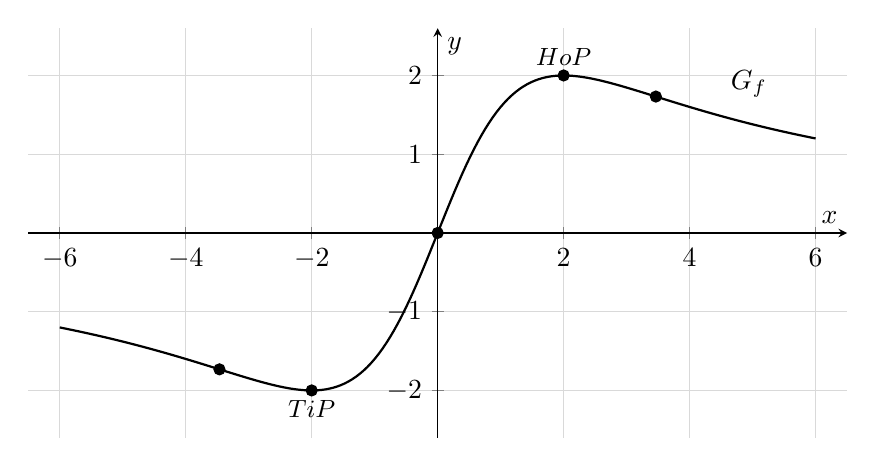
\begin{tikzpicture}
  \begin{axis}[ticklabel style={fill=none}, every tick label/.append style={fill=none},
      axis lines=middle, xmin=-6.5, xmax=6.5, ymin=-2.6, ymax=2.6,
      x=0.8cm, y=1cm, xtick={-6,-4,...,6}, ytick={-2,-1,...,2},
      xlabel=$x$, ylabel=$y$, grid=major, grid style={gray!30}]
    \addplot[thick, samples=200, domain=-6:6]{8*x/(x^2+4)};
    \addplot[only marks, mark=*] coordinates {(2,2) (-2,-2) (0,0) (3.4641,1.7321) (-3.4641,-1.7321)};
    \node[above] at (axis cs:2,2) {\small $HoP$};
    \node[below] at (axis cs:-2,-2) {\small $TiP$};
    \node[above right] at (axis cs:4.5,1.6) {$G_f$};
  \end{axis}
  \end{tikzpicture}
  \end{center}
\end{enumerate}
\end{loesung}

\begin{loesung}{1.35}{Sektglas}
\begin{enumerate}[label=\alph*)]
  \item Volumen von Rotationskörpern:
  \[V(h) = \pi\integral[limits-mode=limits,limits={0, h}]{\left(\sqrt{2x}\right)^2} = \pi\integral[limits-mode=limits,limits={0, h}]{2x} = \pi\left[x^2\right]_0^h = \pi h^2\]
  Volles Glas: $V(8) = 64\pi\approx 201\,\text{cm}^3$, also etwa $201\,\text{ml}$.
  \item $\pi h^2 = 32\pi\Longleftrightarrow h^2 = 32$, wegen $h>0$ also $h = 4\sqrt{2}\approx 5{,}66\,\text{cm}$. Das ist deutlich mehr als die halbe Glashöhe ($4\,\text{cm}$): Das Glas ist unten schmal und oben breit, sodass die untere Hälfte der Höhe nur $V(4) = 16\pi$, also ein Viertel des Volumens, fasst.
  \item Füllzeit: $\dfrac{64\pi\,\text{ml}}{20\,\frac{\text{ml}}{\text{s}}}\approx 10{,}05\,\text{s}$.\\
  Pro Sekunde kommen stets $20\,\text{ml}$ hinzu. Die Änderung des Volumens pro Zentimeter Füllhöhe ist $V'(h) = 2\pi h$ und wächst mit $h$ (der Querschnitt wird größer). Dieselben $20\,\text{ml}$ heben den Spiegel deshalb bei kleiner Füllhöhe stärker an als bei großer.
\end{enumerate}
\end{loesung}

\begin{loesung}{1.36}{Logistisches Wachstum}
\begin{enumerate}[label=\alph*)]
  \item $B(0) = \dfrac{1000}{1+9} = 100$. Für $t\longrightarrow\infty$ gilt $e^{-0{,}5t}\longrightarrow 0$, also $B(t)\longrightarrow\dfrac{1000}{1} = 1000$.\\
  Anfangsbestand $100\,000$ Bakterien, Sättigungsgrenze $1\,000\,000$ Bakterien.
  \item \[\dfrac{1000}{1+9e^{-0{,}5t}} = 500\ \Longleftrightarrow\ 1+9e^{-0{,}5t} = 2\ \Longleftrightarrow\ e^{-0{,}5t} = \dfrac{1}{9}\ \Longleftrightarrow\ t = 2\ln{(9)}\approx 4{,}39\]
  Nach etwa $4{,}39$ Stunden ist die Hälfte der Sättigungsgrenze erreicht.
  \item Kettenregel ($B(t) = 1000\cdot(1+9e^{-0{,}5t})^{-1}$):
  \[B'(t) = -1000\cdot(1+9e^{-0{,}5t})^{-2}\cdot(-4{,}5e^{-0{,}5t}) = \dfrac{4500e^{-0{,}5t}}{(1+9e^{-0{,}5t})^2}\]
  Rechte Seite: Mit $1-\dfrac{B(t)}{1000} = 1-\dfrac{1}{1+9e^{-0{,}5t}} = \dfrac{9e^{-0{,}5t}}{1+9e^{-0{,}5t}}$ folgt
  \[0{,}5\cdot\dfrac{1000}{1+9e^{-0{,}5t}}\cdot\dfrac{9e^{-0{,}5t}}{1+9e^{-0{,}5t}} = \dfrac{4500e^{-0{,}5t}}{(1+9e^{-0{,}5t})^2} = B'(t)\]
  \item Nach c) hängt die Wachstumsrate nur vom Bestand ab: $B' = 0{,}5\cdot B\cdot\left(1-\frac{B}{1000}\right)$. Als Funktion von $B$ ist das eine nach unten geöffnete Parabel mit den Nullstellen $B=0$ und $B=1000$; ihr Scheitel liegt in der Mitte bei $B=500$. Die maximale Wachstumsrate ist
  \[0{,}5\cdot 500\cdot\left(1-\dfrac{500}{1000}\right) = 125\]
  also $125\,000$ Bakterien pro Stunde, erreicht nach b) zur Zeit $t = 2\ln{(9)}\approx 4{,}39$ (Wendestelle von $G_B$).
\end{enumerate}
\end{loesung}

\begin{loesung}{1.37}{Schachtel mit maximalem Volumen}
\begin{enumerate}[label=\alph*)]
  \item Grundfläche $(30-2x)\cdot(16-2x)$, Höhe $x$:
  \[V(x) = x\cdot(30-2x)\cdot(16-2x) = 4x^3-92x^2+480x\]
  Alle Maße müssen positiv sein: $x>0$ und $16-2x>0\Longleftrightarrow x<8$. Also $\mathds{D}_V = ]0;8[$.
  \item $V'(x) = 12x^2-184x+480 = 4\cdot(3x^2-46x+120) = 0$. Mitternachtsformel:
  \[x_{1,2} = \dfrac{46\pm\sqrt{2116-1440}}{6} = \dfrac{46\pm 26}{6}\quad\Longrightarrow\quad x_1 = \dfrac{10}{3},\ x_2 = 12\notin\mathds{D}_V\]
  $V''(x) = 24x-184$, $V''(\frac{10}{3}) = 80-184 = -104<0$: Maximum. Da $V$ an den Rändern von $\mathds{D}_V$ gegen $0$ strebt, ist es das absolute Maximum.
  \[V\left(\dfrac{10}{3}\right) = \dfrac{10}{3}\cdot\dfrac{70}{3}\cdot\dfrac{28}{3} = \dfrac{19600}{27}\approx 725{,}9\]
  Bei $x = \frac{10}{3}\,\text{cm}\approx 3{,}33\,\text{cm}$ ist das Volumen mit etwa $726\,\text{cm}^3$ maximal.
\end{enumerate}
\end{loesung}

\begin{loesung}{1.38}{Tunnelquerschnitt}
\begin{enumerate}[label=\alph*)]
  \item $p(\pm 4) = 4-4 = 0$ und $k(\pm 4) = 4\cos{\left(\pm\frac{\pi}{2}\right)} = 0$: beide Modelle sind am Boden $8\,\text{m}$ breit.\\
  $p$ ist eine nach unten geöffnete Parabel mit Scheitel $(0|4)$; $k$ hat wegen $\cos\leq 1$ den Maximalwert $k(0) = 4$. Beide sind maximal $4\,\text{m}$ hoch.
  \item \[A_p = \integral[limits-mode=limits,limits={-4, 4}]{\left(4-\dfrac{1}{4}x^2\right)} = \left[4x-\dfrac{1}{12}x^3\right]_{-4}^4 = 2\cdot\left(16-\dfrac{16}{3}\right) = \dfrac{64}{3}\approx 21{,}33\]
  \[A_k = \integral[limits-mode=limits,limits={-4, 4}]{4\cos{\left(\dfrac{\pi}{8}x\right)}} = \left[\dfrac{32}{\pi}\sin{\left(\dfrac{\pi}{8}x\right)}\right]_{-4}^4 = \dfrac{64}{\pi}\approx 20{,}37\]
  Die Querschnittsflächen betragen etwa $21{,}33\,\text{m}^2$ bzw. $20{,}37\,\text{m}^2$.
  \item Das Fahrzeug reicht von $x=-1{,}25$ bis $x=1{,}25$. Beide Funktionen sind achsensymmetrisch und fallen für $x>0$ streng monoton, die kritische Stelle ist also die Fahrzeugkante $x = 1{,}25$:
  \[p(1{,}25)\approx 3{,}61>3,\qquad k(1{,}25)\approx 3{,}53>3\]
  Das Fahrzeug passt in beiden Modellen durch den Tunnel.
  \item $p(x) = 3\Longleftrightarrow x^2 = 4\Longleftrightarrow x = \pm 2$: Breite $4\,\text{m}$.\\
  $k(x) = 3\Longleftrightarrow\cos{\left(\frac{\pi}{8}x\right)} = 0{,}75\Longleftrightarrow x = \pm\frac{8}{\pi}\arccos{(0{,}75)}\approx\pm 1{,}84$: Breite etwa $3{,}68\,\text{m}$.
\end{enumerate}
\end{loesung}

\LoesungskapitelEnde
